% figures/review-process.tex
\documentclass[11pt]{article}
\usepackage[margin=1.5cm]{geometry}
\usepackage{tikz}
\usetikzlibrary{positioning,arrows.meta}
\pagestyle{empty}
\begin{document}
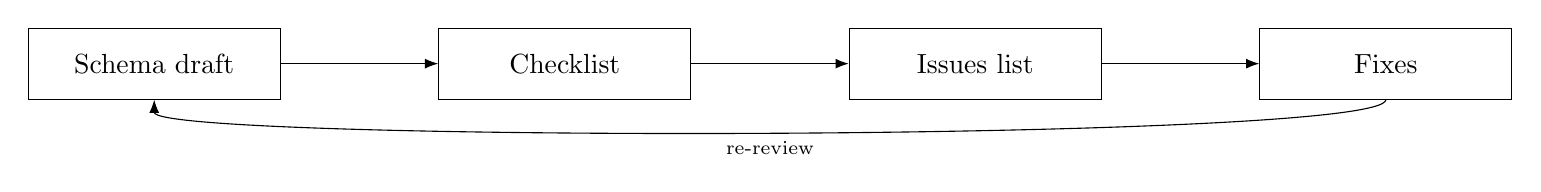
\begin{tikzpicture}[node distance=16mm, >=Latex]
  \node[draw, rectangle, minimum width=3.2cm, minimum height=0.9cm, align=center] (schema) {Schema draft};
  \node[draw, rectangle, minimum width=3.2cm, minimum height=0.9cm, align=center, right=20mm of schema] (check) {Checklist};
  \node[draw, rectangle, minimum width=3.2cm, minimum height=0.9cm, align=center, right=20mm of check] (issues) {Issues list};
  \node[draw, rectangle, minimum width=3.2cm, minimum height=0.9cm, align=center, right=20mm of issues] (fixes) {Fixes};
  \draw[->] (schema) -- (check);
  \draw[->] (check) -- (issues);
  \draw[->] (issues) -- (fixes);
  \draw[->] (fixes) .. controls +(0,-1.0) and +(0,-1.0) .. (schema) node[midway, below, font=\scriptsize] {re-review};
\end{tikzpicture}
\end{document}
